% \documentclass{book}

\documentclass[12pt]{article}
\usepackage[pdfborder={0 0 0.5 [3 2]}]{hyperref}%
\usepackage[left=1in,right=1in,top=1in,bottom=1in]{geometry}%
\usepackage[shortalphabetic]{amsrefs}%
\usepackage{amsmath}
\usepackage{enumerate}
\usepackage{enumitem}
\usepackage{amssymb}                
\usepackage{amsmath}                
\usepackage{amsfonts}
\usepackage{amsthm}
\usepackage{bbm}
\usepackage[table,xcdraw]{xcolor}
\usepackage{tikz}
\usepackage{float}
\usepackage{booktabs}
\usepackage{svg}
\usepackage{mathtools}
\usepackage{cool}
\usepackage{url}
\usepackage{graphicx,epsfig}
\usepackage{makecell}
\usepackage{array}

\def\noi{\noindent}
\def\T{{\mathbb T}}
\def\R{{\mathbb R}}
\def\N{{\mathbb N}}
\def\C{{\mathbb C}}
\def\Z{{\mathbb Z}}
\def\P{{\mathbb P}}
\def\E{{\mathbb E}}
\def\Q{\mathbb{Q}}
\def\ind{{\mathbb I}}

\graphicspath{ {images7/} }

\begin{document}

\section*{26 Feb 2017}
It turns out we had a small error in our exponential weight linearization. Before we get to that, we will first settle a few other small issues.

\subsection*{What mesh sizes do we need?}
For this, we take domain size $L = 50$ and $c = 6.2570$. We use the first double pulse, since it has real eigenvalues of largest magnitude. First, we have Fourier spectral methods with $N = 1024$ (Fourier is always periodic BCs). Here is the plot of eigenvalues of the linearization about the first double pulse.

\begin{figure}[H]
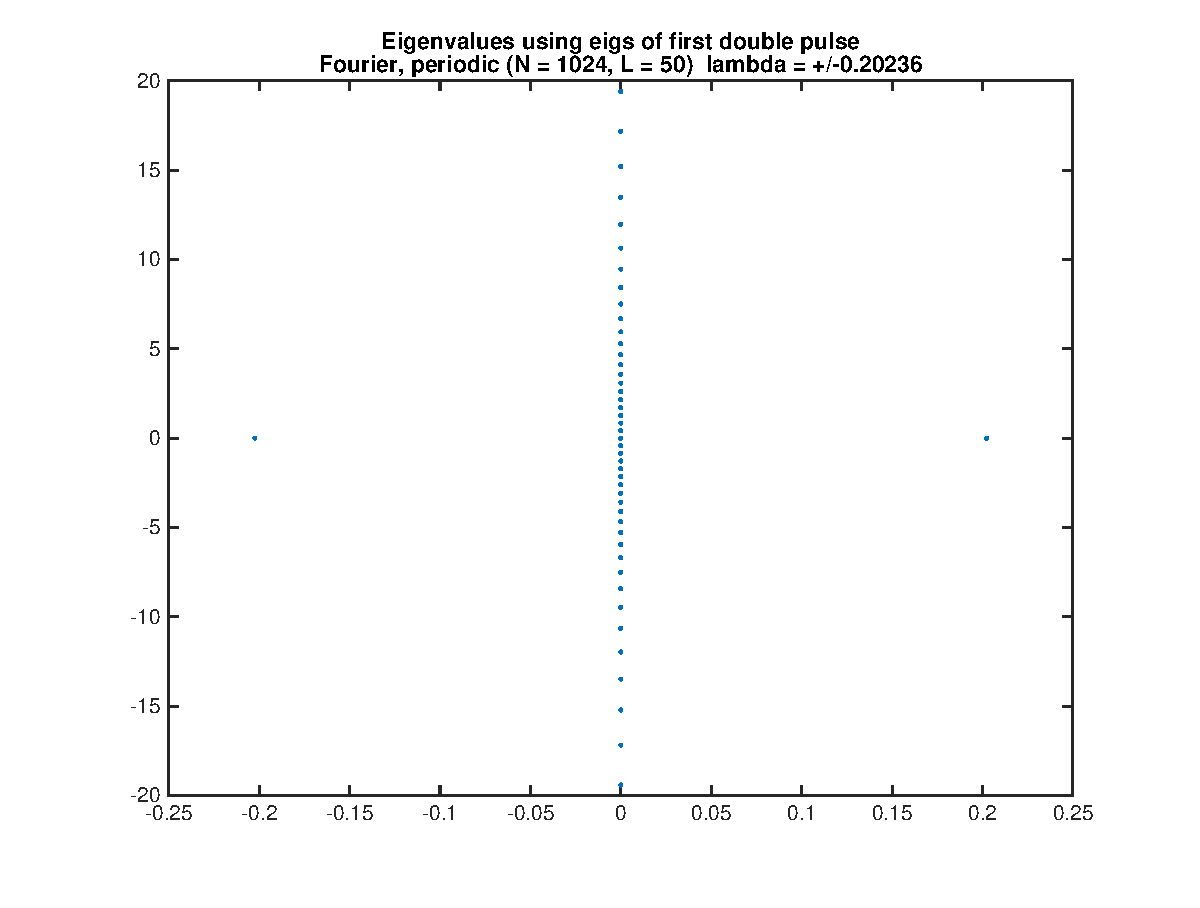
\includegraphics[width=8.5cm]{d1fouriereig.eps}
\end{figure}

As expected, we have a pair of real eigenvalues $(\lambda = \pm 0.20236)$ which are negatives of each other, and the eigenfunctions are localized (not shown), so this is good, i.e. 1024 grid points should be sufficient.\\

Now let's do finite difference method with Neumann BCs. Here we use $L = 50$ and $N = 1000$. Here is a plot of the eigenvalues for the finite difference case. 

\begin{figure}[H]
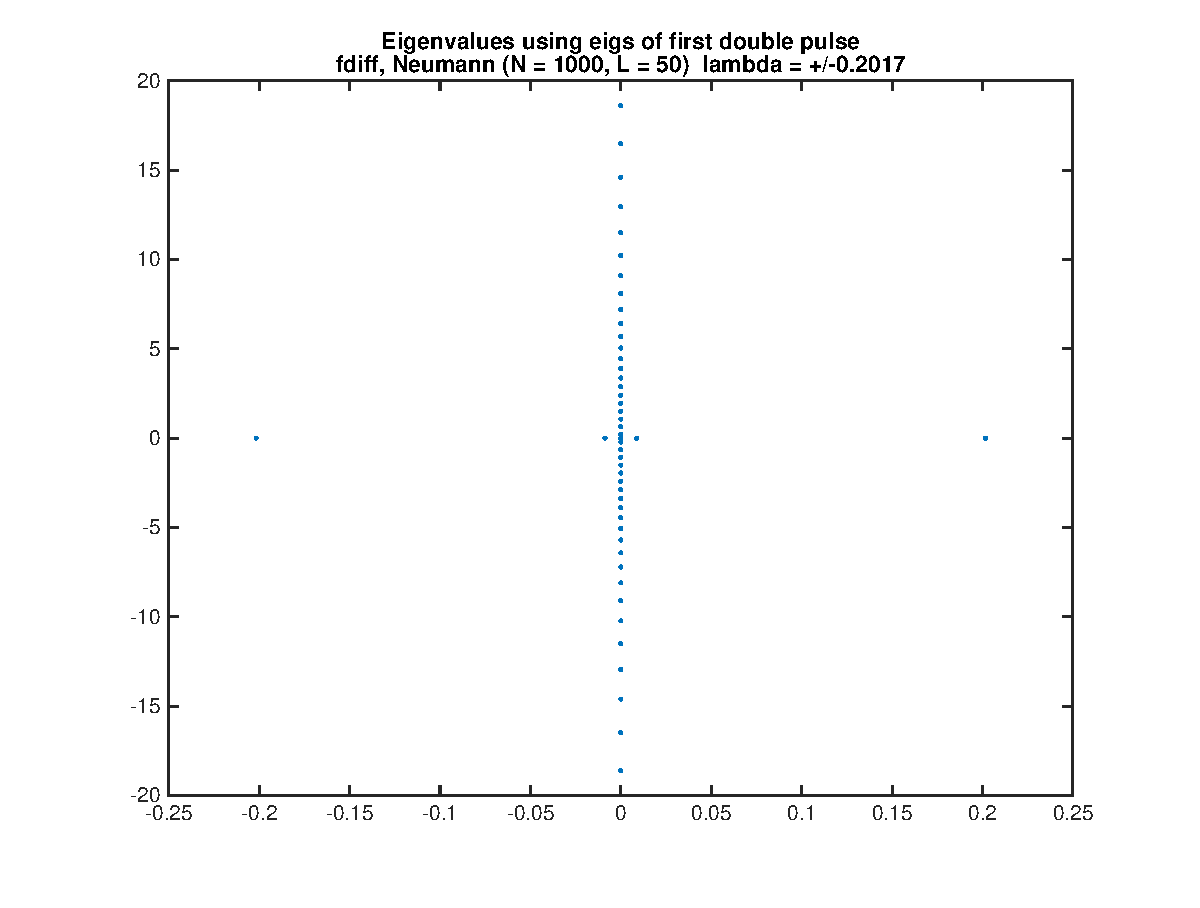
\includegraphics[width=8.5cm]{d1fdiffeig1000.eps}
\end{figure}

We have a pair of real eigenvalues $(\lambda = \pm 0.2017)$ similar to above. We also have another pair of small eigenvalues flanking the origin $(\lambda = \pm 0.0088)$. Are these real or numerical artifact? The eigenfunction looks like the derivative of the double pulse for both of them, so we suspect they are numerical artifact, i.e. should be zero. To support this claim, we increase the number of grid points and see what happens. Here is a plot of the same thing for $N = 5000$.

\begin{figure}[H]
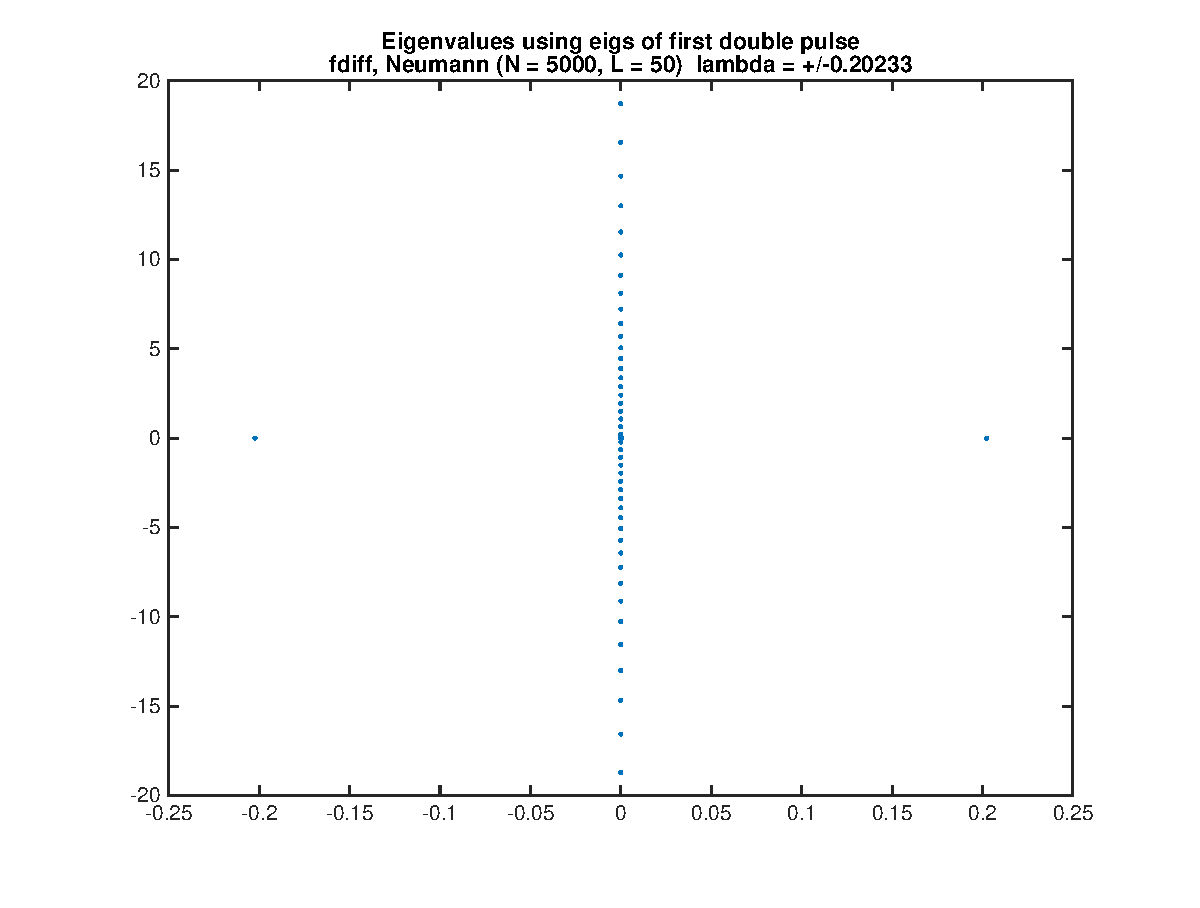
\includegraphics[width=8.5cm]{d1fdiffeig5000.eps}
\end{figure}

The first pair of eigenvalues is approaching the Fourier case above, while the second, smaller pair is approaching 0. Here is a plot of the log of the smaller eigenvalue versus the log of the mesh size. For this plot, ``error'' means size of eigenvalue, since we are assuming the true eigenvalue is 0.

\begin{figure}[H]
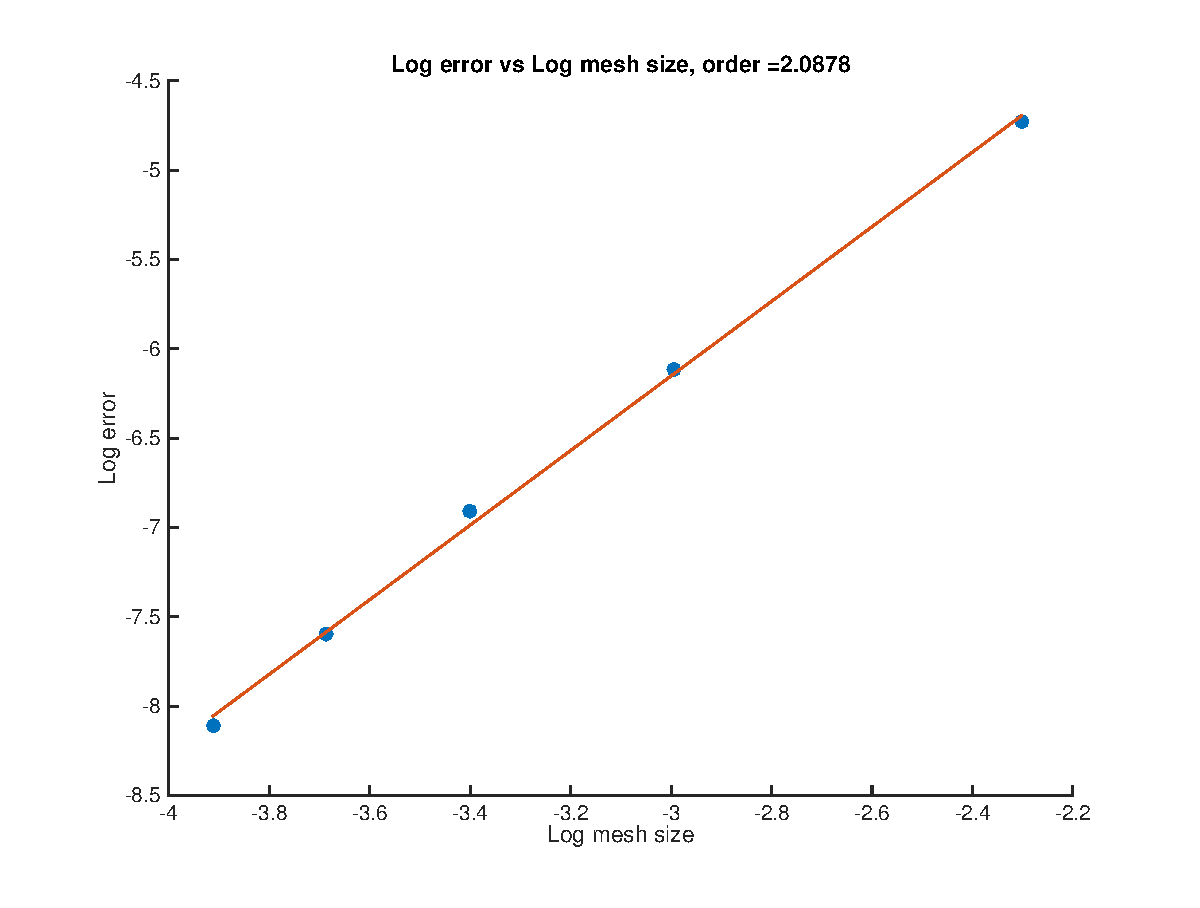
\includegraphics[width=8.5cm]{smalleigerror.eps}
\end{figure}

From this, we see that we have convergence of the small eigenvalue to 0 with 2nd order accuracy. This makes sense since we are using a 2nd order method. Thus we can safely ignore this small eigenvalue pair. For $L = 50$ we should use at least 5000 grid points, i.e a mesh size no larger than 0.0200.

\subsection*{Linearization about the zero solution}
Now we move to an exponentially weighed space, with weight $a$. The differentiation operator $\partial_x$ becomes $\partial_x - a$, otherwise everything is unchanged. (Could have a positive sign there, but it does not matter).\\

If we linearize about the zero function $u^* = 0$, what happens? The derivative $u^*_x$ is still the zero function, but the zero function is not an eigenfunction, so we do not have an eigenfunction with eigenvalue 0.\\

In the weighted space, the constant function (say, $v = 1$) also solves the eigenvalue problem with eigenvalue:
\[ 
\lambda = -a^5 + a^3 - c a 
\]
This function is not in $L^2$ nor any weighted $L^2$, so it is not actually an eigenfunction. However, if we restrict to a finite domain, it is an eigenfunction, and it satisfies Neumann BCs, so we expect to see it for that discretization. Let's check for $a = 0.01$.

\begin{figure}[H]
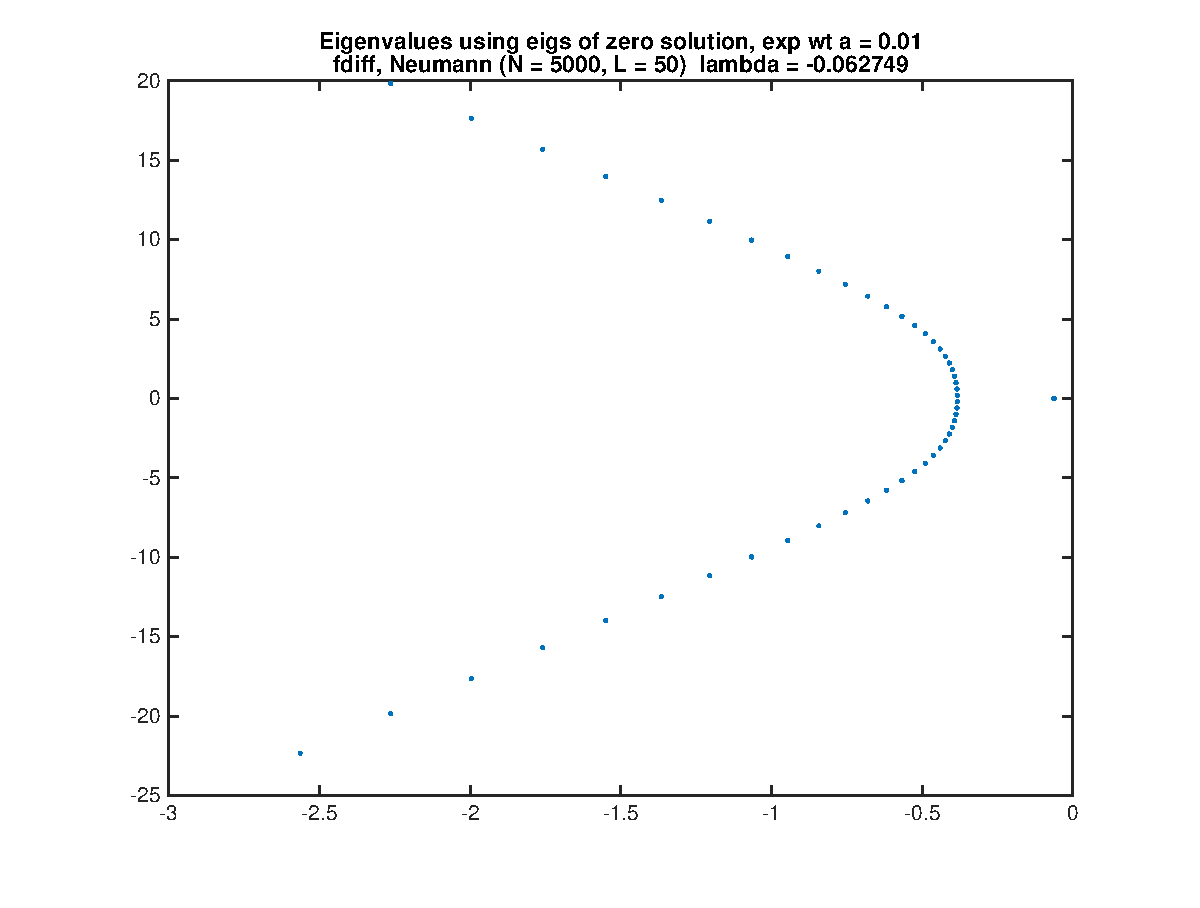
\includegraphics[width=8.5cm]{zeroeigsfdiff.eps}
\end{figure}
The exponential spectrum is moved to the left, and we have a single eigenvalue at $\lambda = -0.0627$, which agrees with our formula above. The corresponding eigenfunction is a constant function. Changing the exponential weight $a$ still produces the correct eigenvalue.\\

How about Fourier?
\begin{figure}[H]
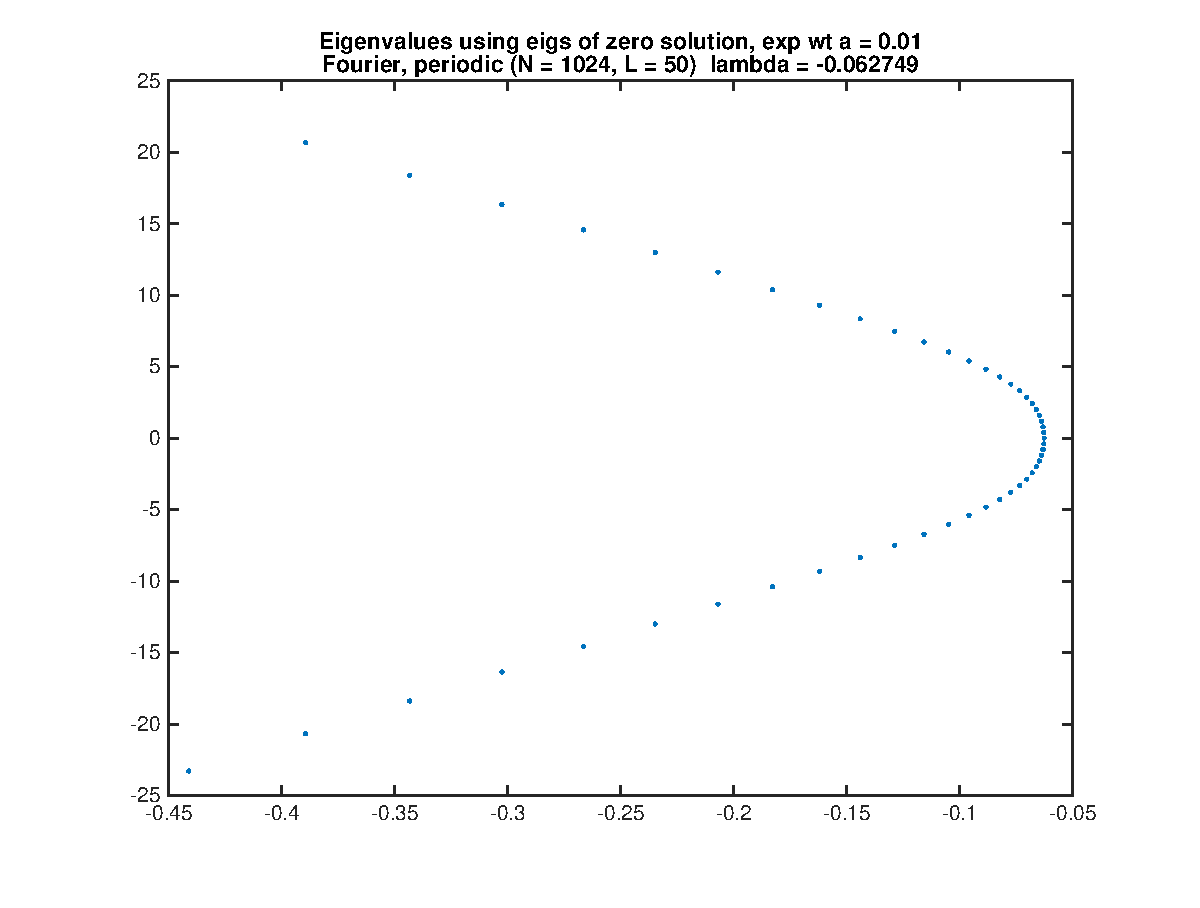
\includegraphics[width=8.5cm]{zeroeigsfourier.eps}
\end{figure}
It doesn't look like it is there, but is there! In fact, the eigenvalue $\lambda = -0.0627$ is at the tip of the essential spectrum. If we check the corresponding eigenfunction, it is the constant function. If we change the weight $a$, we still get the correct eigenvalue at the tip of the essential spectrum.\\

Looking at the two plots above, the exponential weight separates the constant eigenvalue from the essential spectrum only in the finite difference/Neumann case. Not really sure why this is true.

\subsection*{Try this on actual double pulses}
Now we try this on actual double pulses. We did this earlier, but I found a coding error. The linearization about a solution $u^*$ of the 5th order KdV is:
\[
J = \partial_x^5 - \partial_x^3 + c \partial_x - 2 u^*_x - 2 u^* \partial_x
\]
If we move this to an exponentially weighted space (weight $a$), this becomes:
\[
J_a = (\partial_x - a)^5 - (\partial_x - a)^3 + c (\partial_x - a) - 2 u^*_x - 2 u^* (\partial_x-a)
\]
The derivative of the solution $u^*_x$ is taken with the regular differentation operator, not the weighted operator $\partial_x - a$. We had this wrong in all previous numerics.\\

Now that we have the operator correct, let's do this on double pulses 2, 4, and 6 for Fourier. (These are the double pulses are are interested in, since we already know what's up for double pulses 1, 3, and 5). We would like an exponential weight $a$ which provides the maximum separation of the essential spectrum from the point spectrum. One way to find an ``ideal'' $a$ is to look at the temporal eigenvalues of the spatial eigenvalue problem of the linearization about the zero function. As the spatial eigenvalue $\lambda$ is increased, the temporal eigenvalue at 0 moves to the right, and the rightmost temporal eigenvalues move to the left. We can compute numerically where the real part of these eigenvalues meet (at $\lambda$ is increased.) For this value of $c$, we compute an ``ideal'' $a = 0.9318$. This turns out to be a bit too large, but we will, say, approximately cut this in half and use $a = 0.5$. This provides good separation, so it will do for now.\\

Here's what we get. In all cases, there are 4 eigenvalues away from the essential spectrum (which si what we expect). Zooms are provided.

\begin{figure}[H]
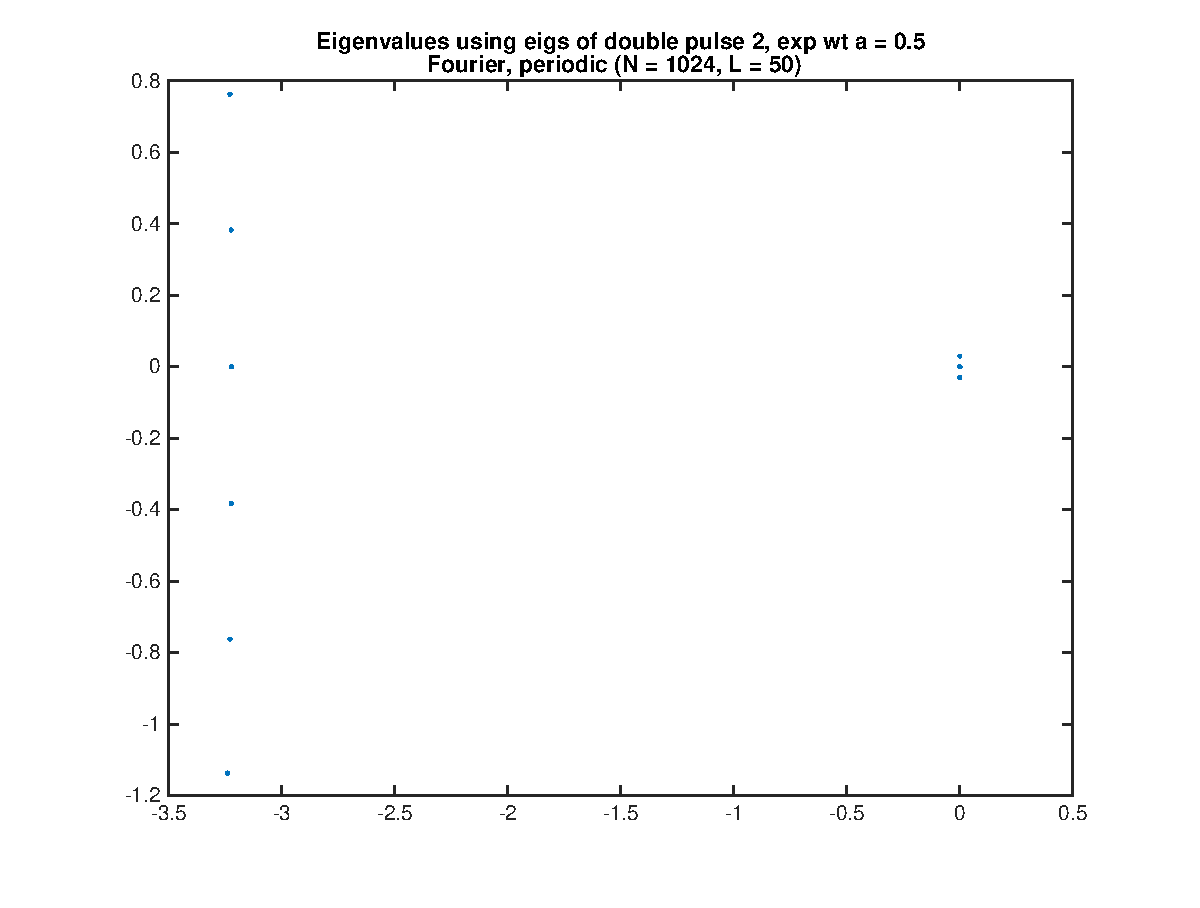
\includegraphics[width=8.5cm]{fourierD2eigs.eps}
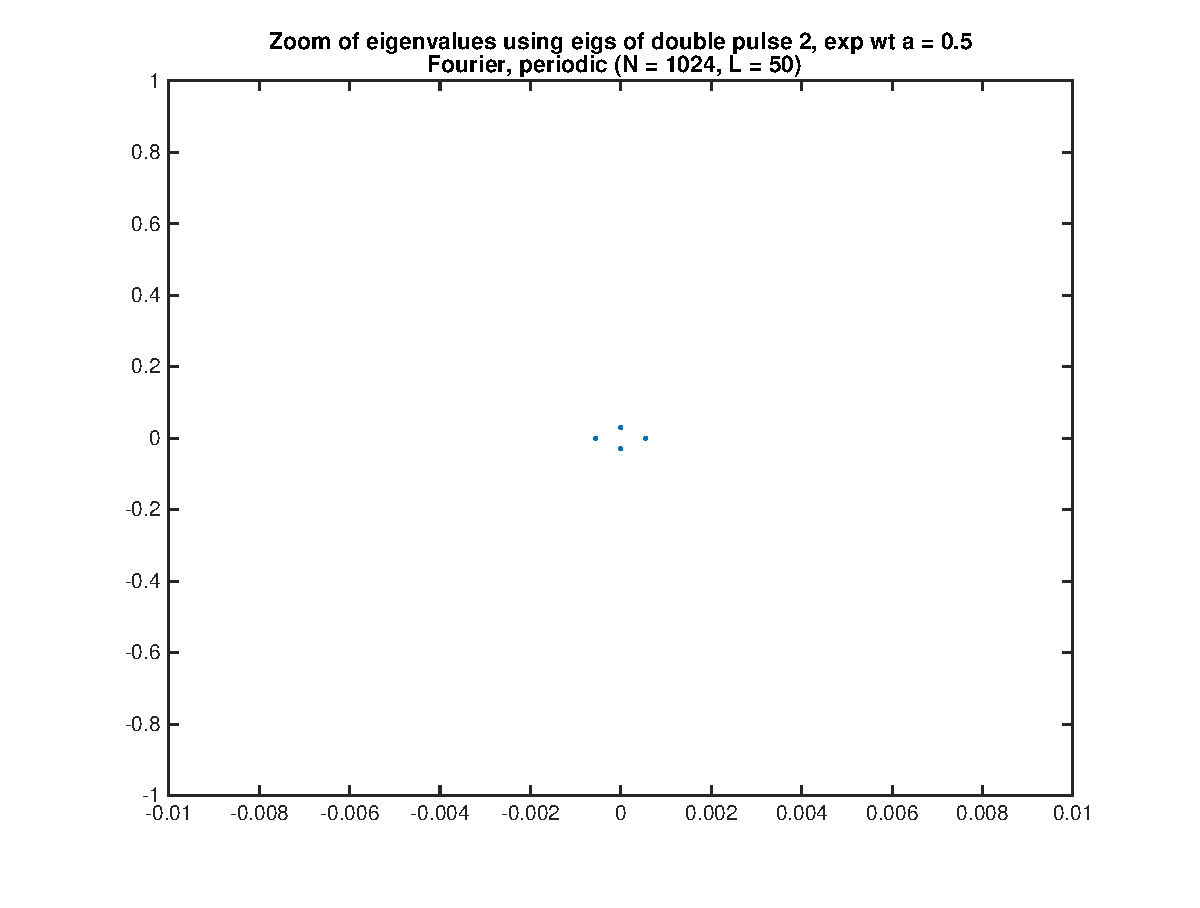
\includegraphics[width=8.5cm]{fourierD2eigszoom.eps}
\end{figure}
\begin{figure}[H]
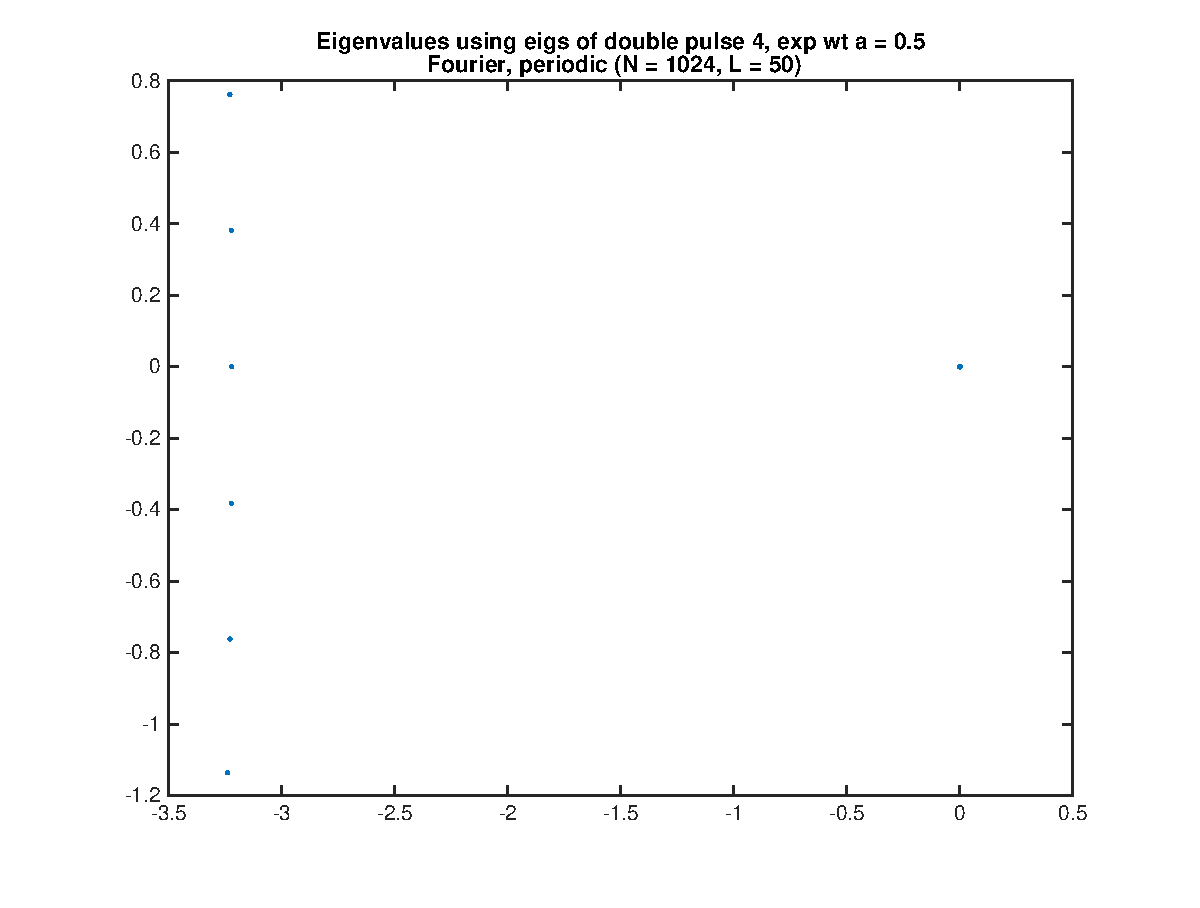
\includegraphics[width=8.5cm]{fourierD4eigs.eps}
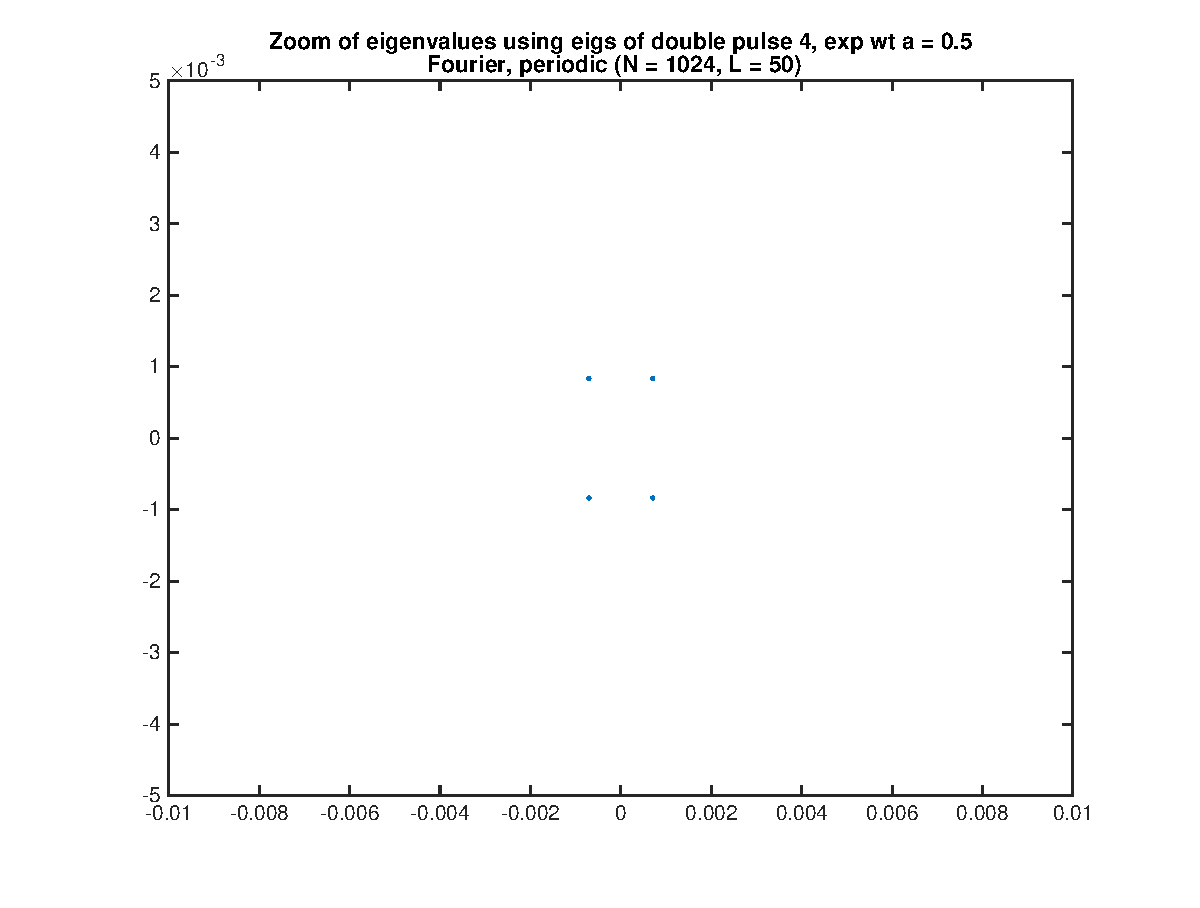
\includegraphics[width=8.5cm]{fourierD4eigszoom.eps}
\end{figure}
\begin{figure}[H]
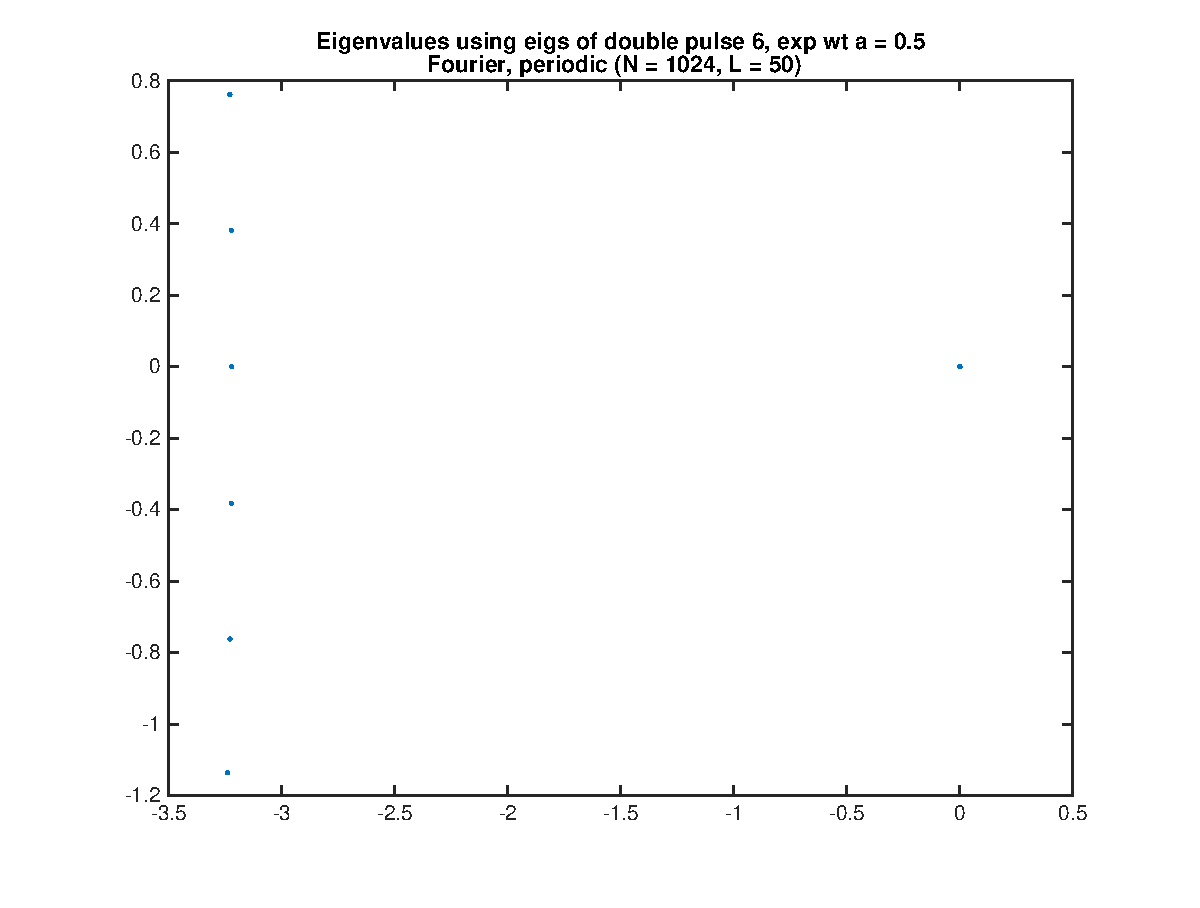
\includegraphics[width=8.5cm]{fourierD6eigs.eps}
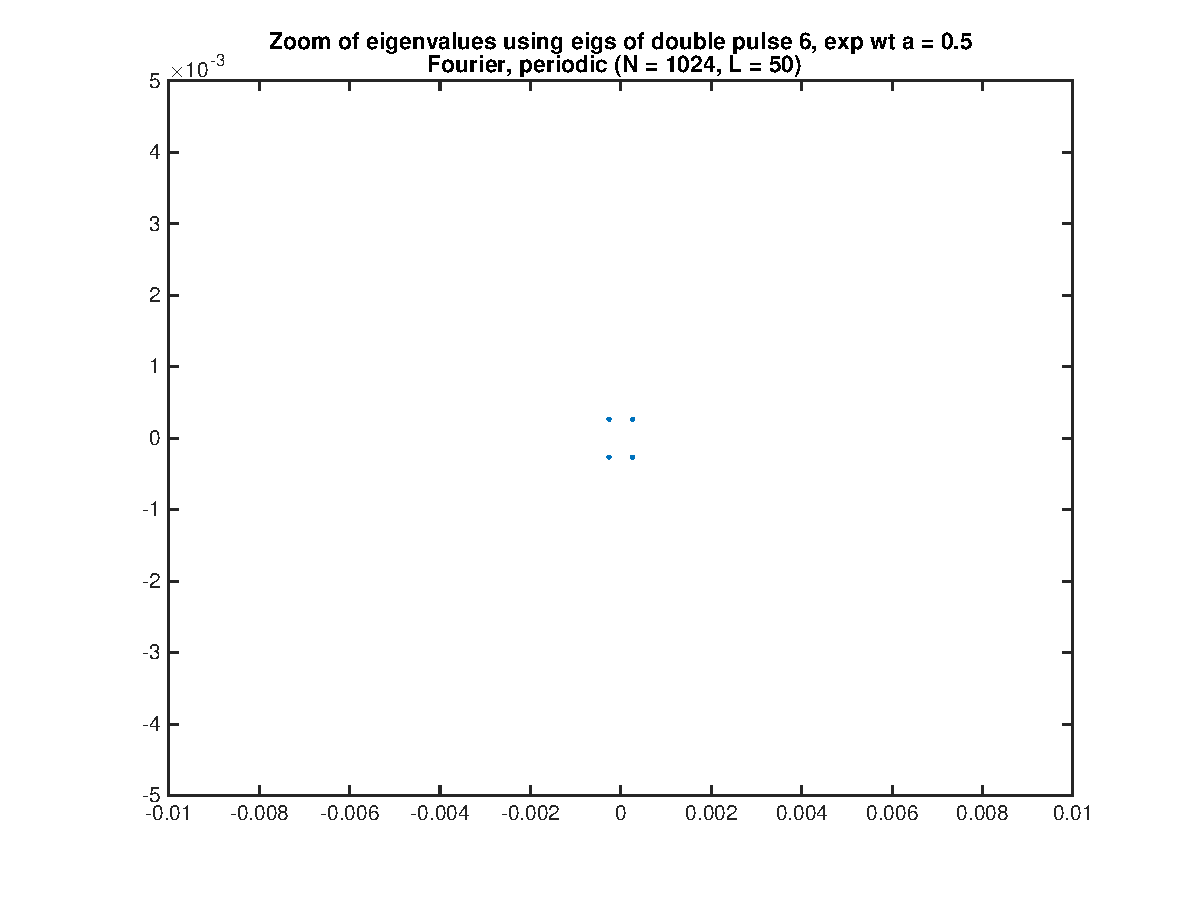
\includegraphics[width=8.5cm]{fourierD6eigszoom.eps}
\end{figure}

Table of eigenvalues:
\begin{figure}[H]
\begin{tabular}{l|lll}
Eigenvalue & Double pulse 2 & Double pulse 4 & Double pulse 6  \\ \hline
      &                     &  1.0e-3 *             & 1.0e-3 * \\
1     &    0.0000 - 0.0296i &     0.7310 - 0.8568i  &    0.2633 - 0.2681i      \\
2     &    0.0000 + 0.0296i &     0.7310 + 0.8568i  &    0.2633 + 0.2681i      \\
3     &    0.0005 + 0.0000i &    -0.7310 - 0.8579i  &   -0.2633 - 0.2682i      \\
4     &   -0.0005 + 0.0000i &    -0.7310 + 0.8579i  &   -0.2633 + 0.2682i      \\       
\end{tabular}
\end{figure}

Here is a plot of the log of the imaginary part of the eigenvalues versus spacing between the pulses.
\begin{figure}[H]
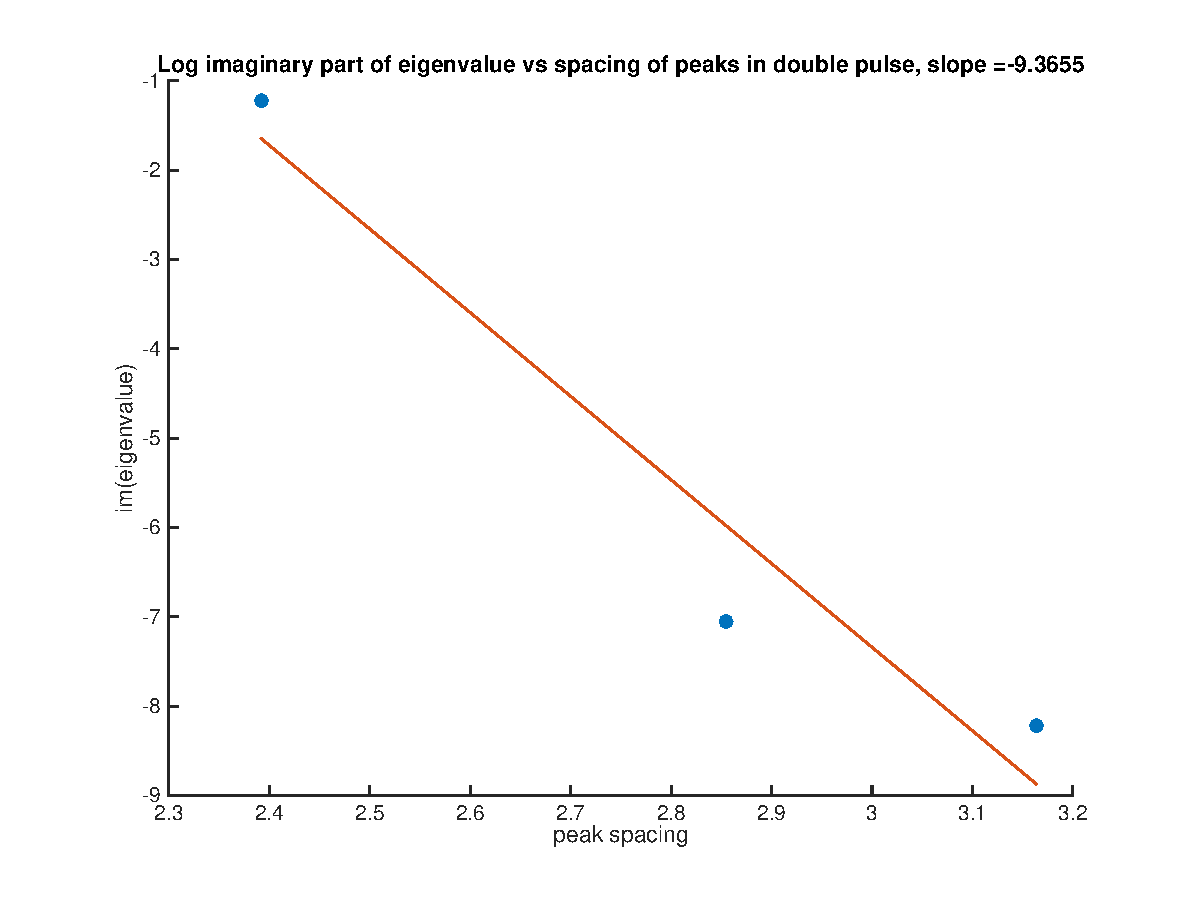
\includegraphics[width=8.5cm]{logimagspacing.eps}
\end{figure}
We only have 3 data points, but it's only an okay straight line. Let's construct one more double pulse (double pulse 8). I don't want to go too much further, since the periodic boundary might start to be a problem, and increasing the domain size will mean we have to increase the number of Fourier nodes, which is slow.

\begin{figure}[H]
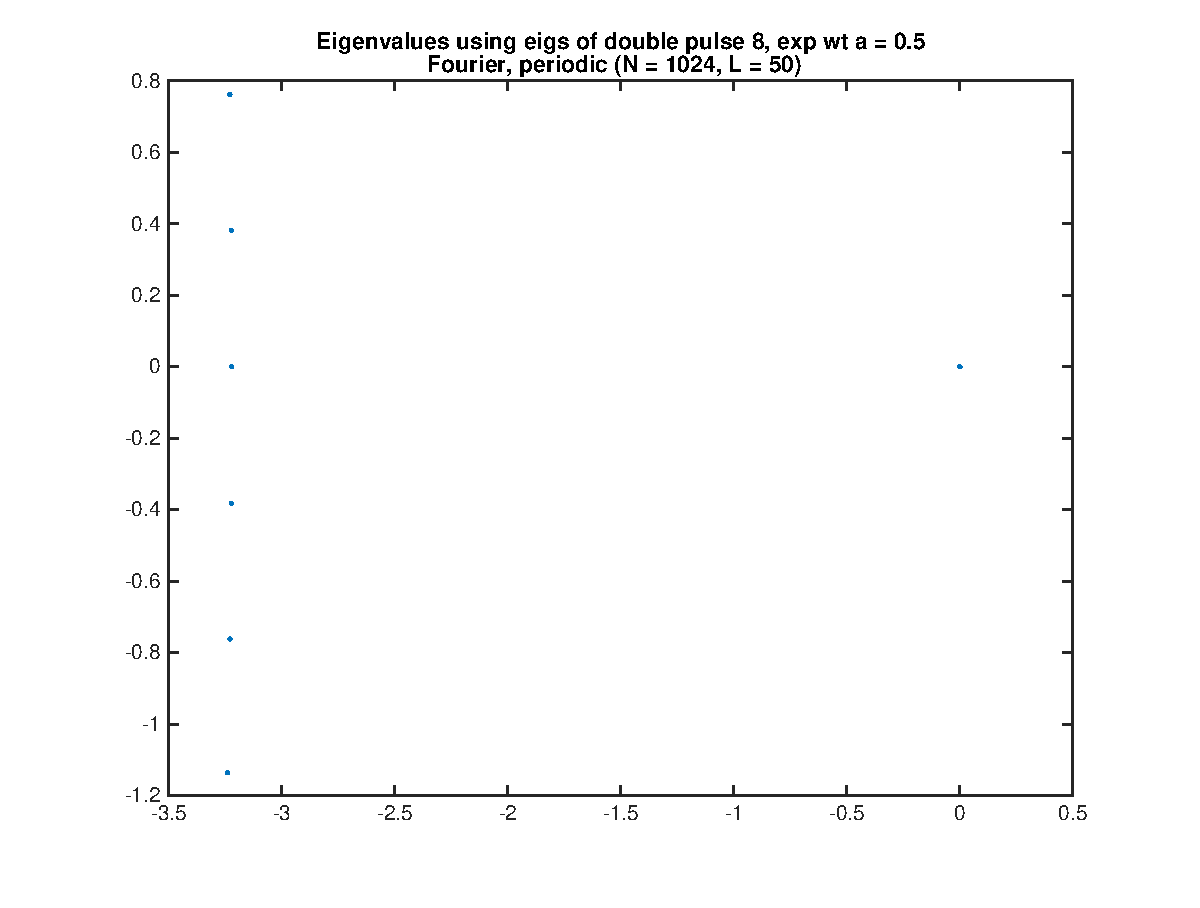
\includegraphics[width=8.5cm]{fourierD8eigs.eps}
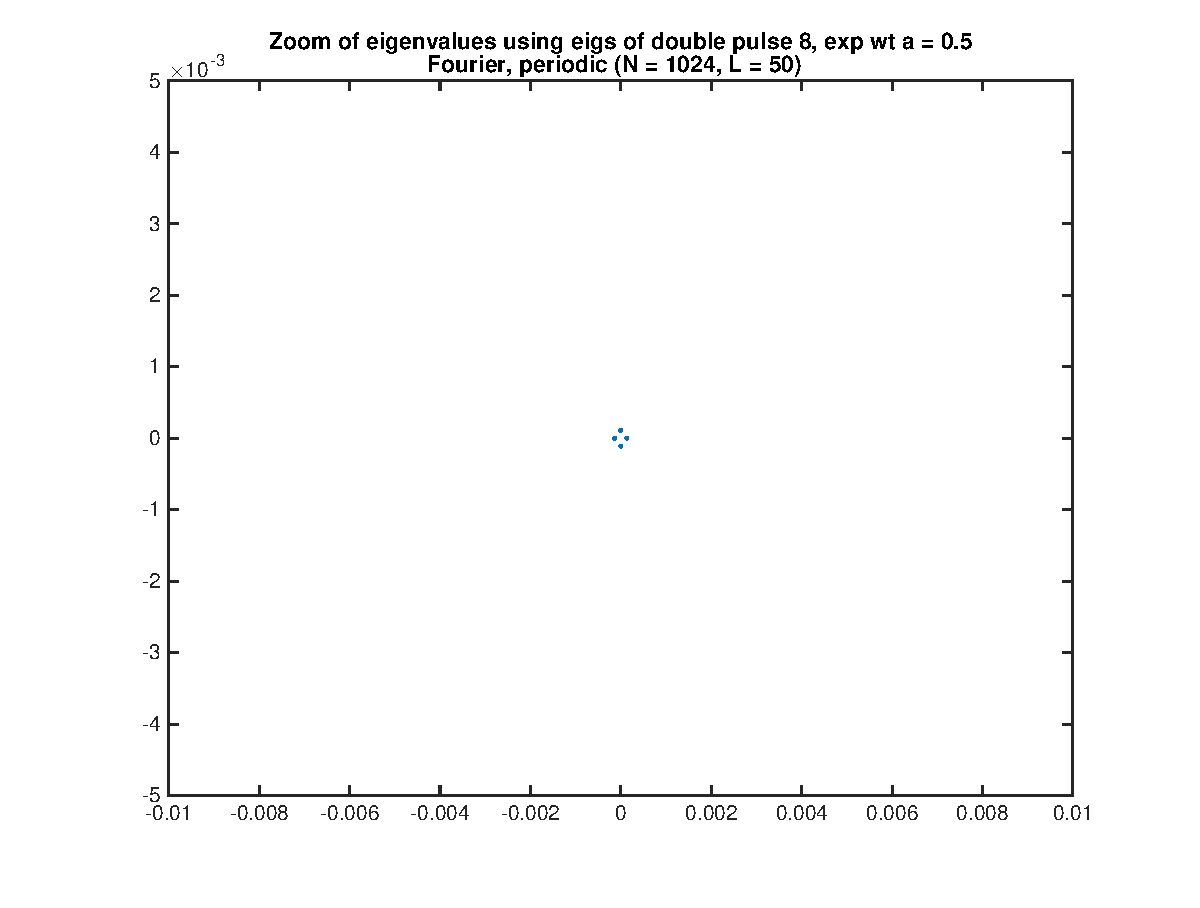
\includegraphics[width=8.5cm]{fourierD8eigszoom.eps}
\end{figure}

Repeating the log plot:
\begin{figure}[H]
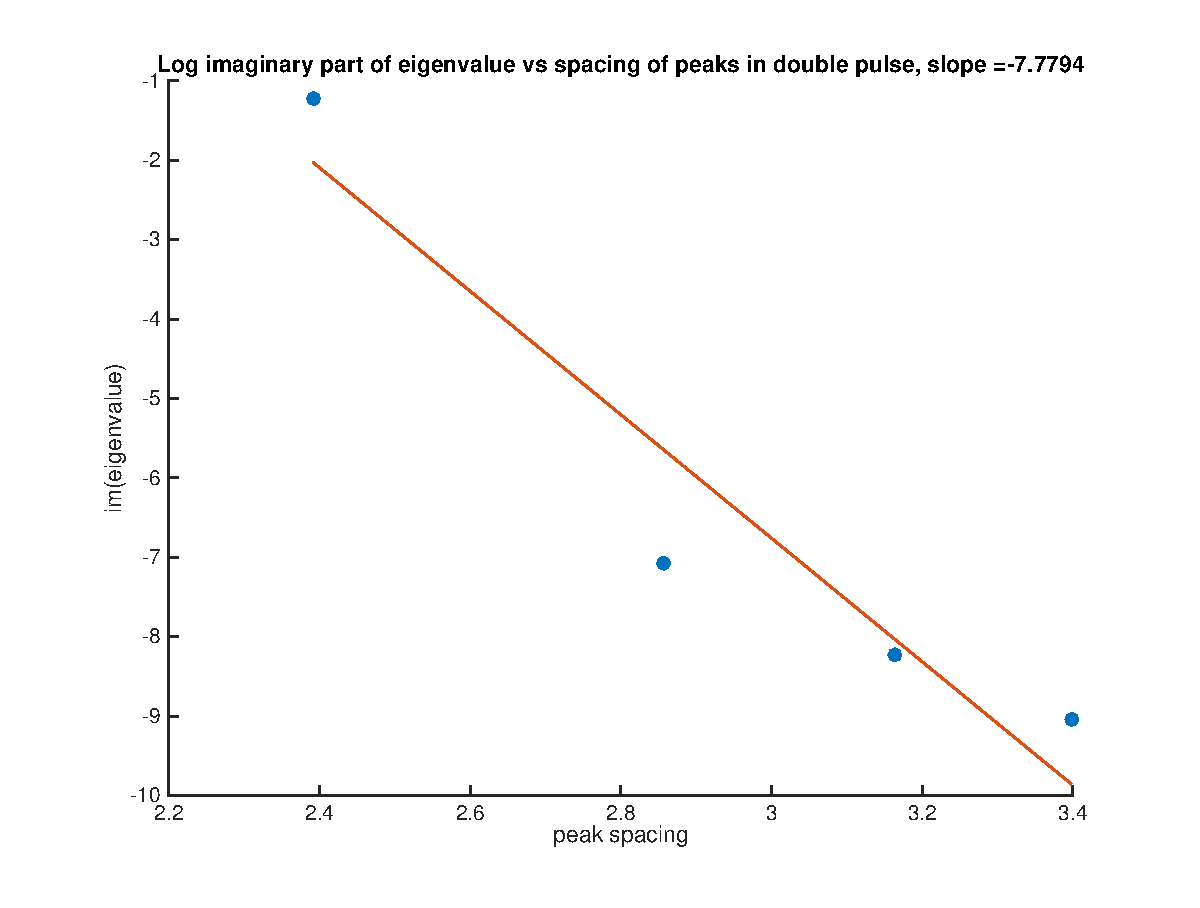
\includegraphics[width=8.5cm]{logimagspacing2.eps}
\end{figure}
This would look nice if you ditch the first point.\\

If you look at the zoom eigenvalue plot, we have a diamond, followed by two rectangles, followed by a diamond. No idea why. Or even if this is correct. All eigenfunctions are localized.\\

What happens if we increase number of grid points? For $N = 2048$ we have:

Table of eigenvalues:
\begin{figure}[H]
\begin{tabular}{l|llll}
Eigenvalue & Double pulse 2 & Double pulse 4 & Double pulse 6  & Double pulse 8 \\ \hline
1     &    0.0000 - 0.0043i &   0.0018 - 0.0019i &    0.0005 - 0.0006i  &    0.0000 - 0.0003i  \\
2     &    0.0000 + 0.0043i &   0.0018 + 0.0019i &    0.0005 + 0.0006i  &    0.0000 + 0.0003i  \\
3     &    0.0000 - 0.0293i &  -0.0018 - 0.0019i &   -0.0005 - 0.0006i  &    0.0001 + 0.0000i  \\
4     &    0.0000 + 0.0293i &  -0.0018 + 0.0019i &   -0.0005 + 0.0006i  &   -0.0001 + 0.0000i  \\       
\end{tabular}
\end{figure}

Except for the Double Pulse 2, the eigenvalues are similar to the $N = 1024$ case in configuration. For Double Pulse 2, the larger magnitude pair is approximately in the same place, although the other pair has shifted from real axis to imaginary axis. The decay plot for these looks similar to the case for $N = 1024$.

\subsection*{Finite Differences with Neumann BCs}
What happens with finite difference/Neumann BCs. Same $c$ and exp st $a = 0.5$ as above. For the second double pulse and $N = 5000$, plot looks like:
\begin{figure}[H]
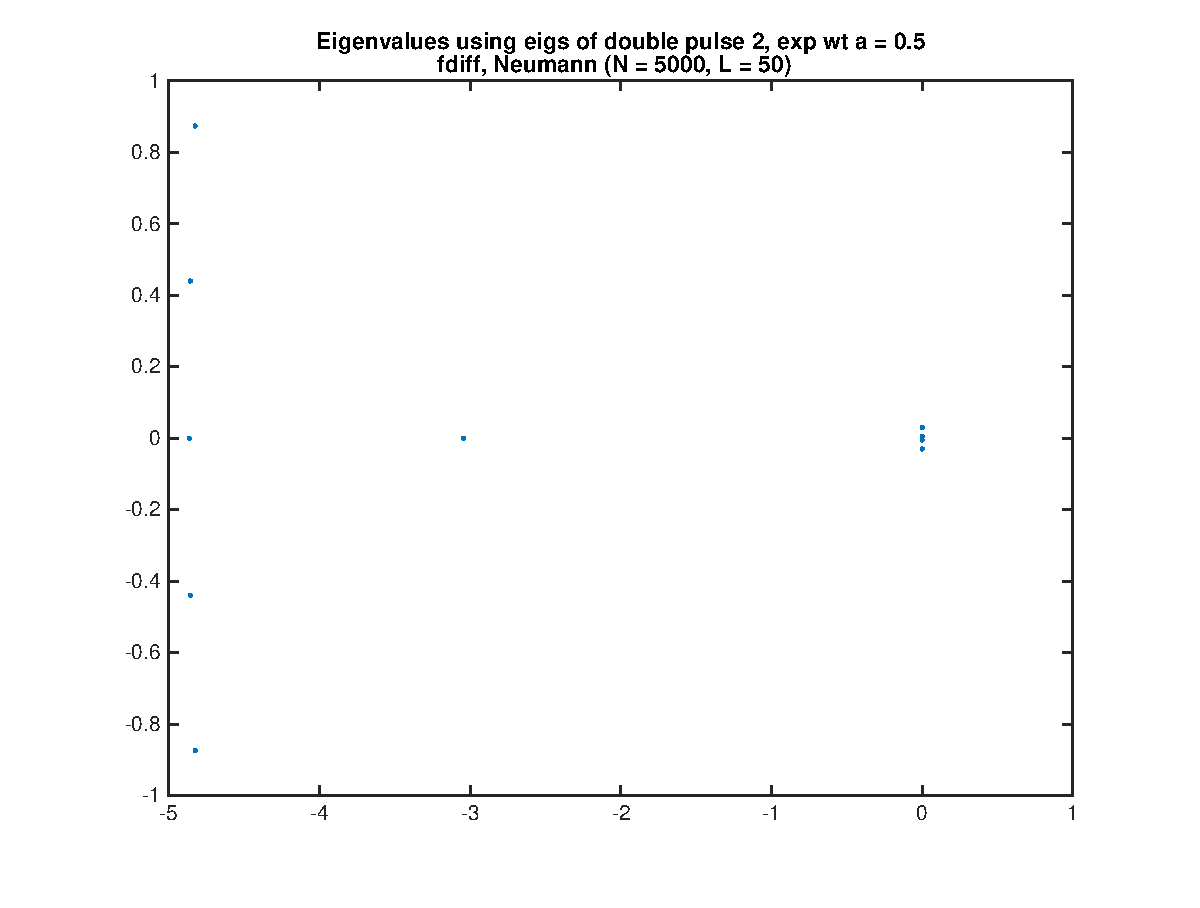
\includegraphics[width=8.5cm]{fd5000eigs.eps}
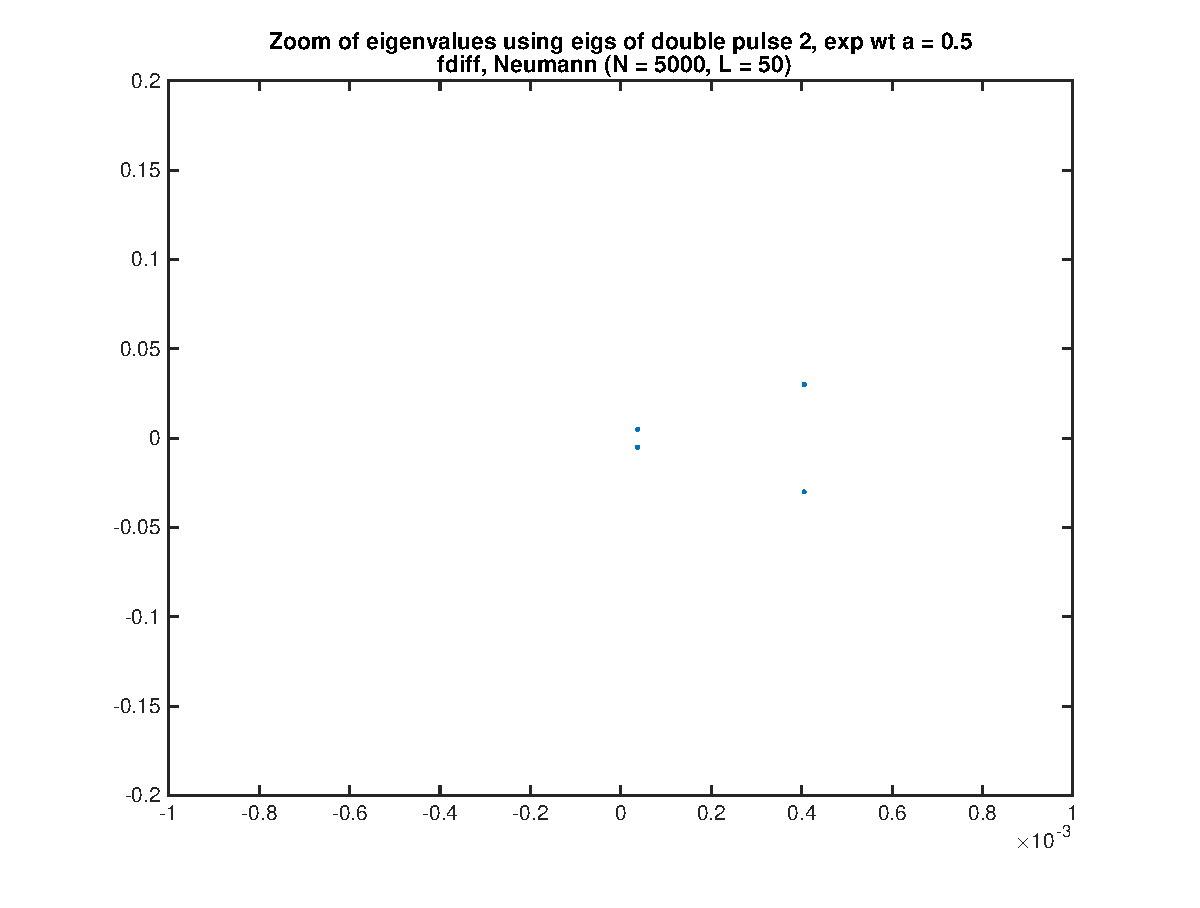
\includegraphics[width=8.5cm]{fd5000eigszoom.eps}
\end{figure}
In addition to a cluster of 4 eigenvalues as expected, we also have an eigenvalue at $\lambda = -3.0438$, which corresponds exactly to the eigenvalue of the constant function when we linearize about the zero solution. If we take $N = 10000$, the eigenvalues are:
\begin{figure}[H]
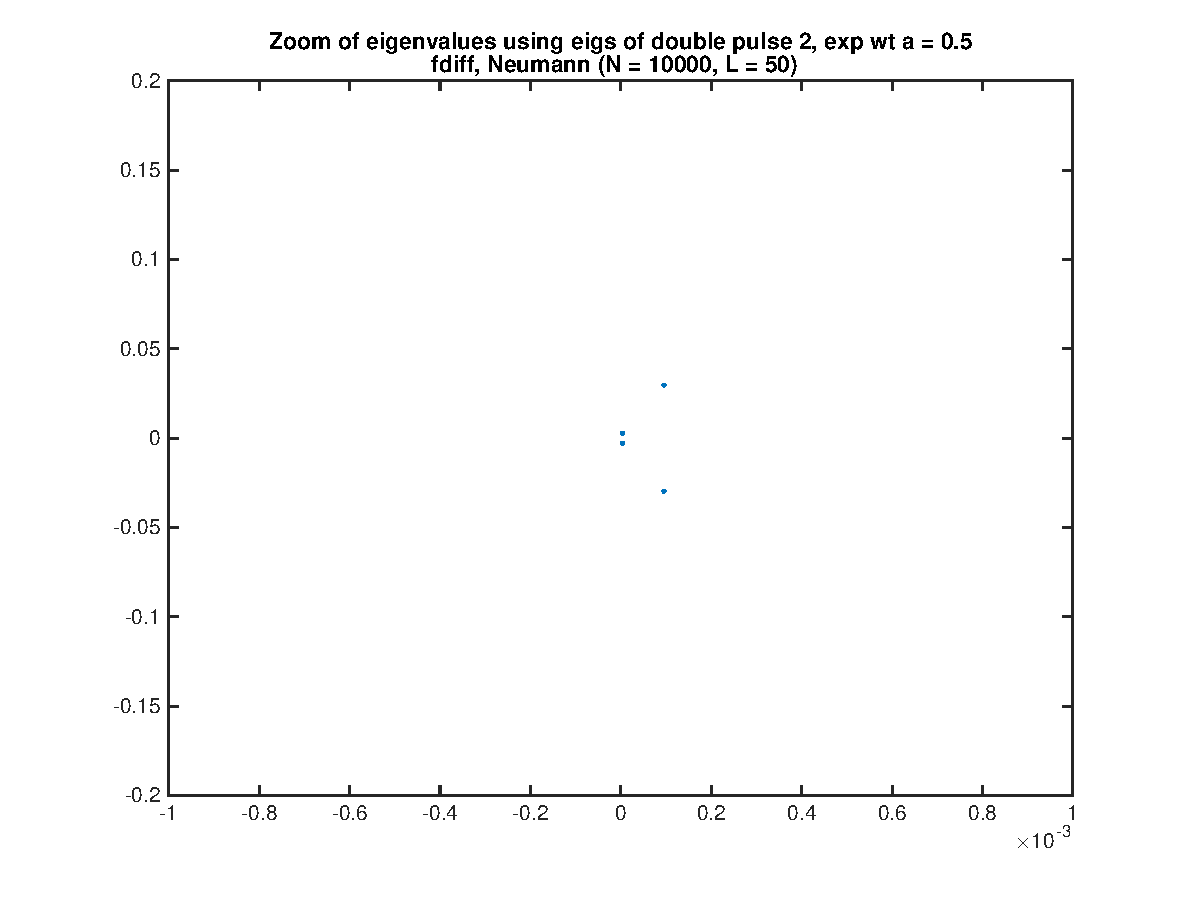
\includegraphics[width=8.5cm]{fd10000eigszoom.eps}
\end{figure}
In table form:
\begin{figure}[H]
\begin{tabular}{l|lll}
Eigenvalue & $N = 5000$ & $N = 10000$  & $N = 15000$\\ \hline
1     &       0.0000 - 0.0050i &     0.0000 - 0.0028i    &  0.0000 - 0.0011i\\
2     &       0.0000 + 0.0050i &     0.0000 + 0.0028i    &  0.0000 + 0.0011i\\
3     &       0.0004 - 0.0301i &     0.0001 - 0.0297i    &  0.0001 - 0.0295i\\
4     &       0.0004 + 0.0301i &     0.0001 + 0.0297i    &  0.0001 + 0.0295i\\       
\end{tabular}
\end{figure}
It looks like we are approaching the Fourier case as the number of grid points increases, so this is good at least. For the other double pulses, it does not look like the Fourier case at all, and the eigenvalue locations seem to be governed by the mesh size. In all cases, there is an eigenvalue at $\lambda = -3.0438$, as we saw above.

\subsection*{More Fourier nodes}
It seems like the results vary with the number of Fourier nodes we use, especially for the smaller eigenvalues. Let's explore that. In all cases, we use Fourier spectral method with $L = 50$ and exp weight $a = 0.5$.

\begin{enumerate}

\item Double pulse 2
\begin{figure}[H]
\begin{tabular}{l|lll}
Eigenvalue & $N = 1024$ & $N = 2048$  & $N = 4000$\\ \hline
           &                    &                    &                      \\
1          &   0.0000 - 0.0296i &   0.0000 - 0.0043i &     0.0001 - 0.0105i \\
2          &   0.0000 + 0.0296i &   0.0000 + 0.0043i &     0.0001 + 0.0105i \\
3          &   0.0006 + 0.0000i &  -0.0000 - 0.0293i &    -0.0001 - 0.0280i \\
4          &  -0.0006 + 0.0000i &  -0.0000 + 0.0293i &    -0.0001 + 0.0280i \\       
\end{tabular}
\end{figure}

\item Double pulse 4
\begin{figure}[H]
\begin{tabular}{l|lll}
Eigenvalue & $N = 1024$ & $N = 2048$  & $N = 3000$\\ \hline
           &    1e-3 *            &                    &                      \\
1          &     0.6888 - 0.8219i &   0.0011 - 0.0012i &   0.0034 - 0.0034i \\
2          &     0.6888 + 0.8219i &   0.0011 + 0.0012i &   0.0034 + 0.0034i \\
3          &    -0.6888 - 0.8216i &  -0.0011 - 0.0012i &  -0.0034 - 0.0034i \\
4          &    -0.6888 + 0.8216i &  -0.0011 + 0.0012i &  -0.0034 + 0.0034i \\       
\end{tabular}
\end{figure}

\item Double pulse 6
\begin{figure}[H]
\begin{tabular}{l|lll}
Eigenvalue & $N = 1024$ & $N = 2048$  & $N = 3000$\\ \hline
           &                    &    1e-3 *           &                      \\
1          &     0.0003 - 0.0003i &    0.5156 - 0.5872i &     0.0001 - 0.0105i \\
2          &     0.0003 + 0.0003i &    0.5156 + 0.5872i &     0.0001 + 0.0105i \\
3          &    -0.0003 - 0.0003i &   -0.5156 - 0.5877i &    -0.0001 - 0.0280i \\
4          &    -0.0003 + 0.0003i &   -0.5156 + 0.5877i &    -0.0001 + 0.0280i \\       
\end{tabular}
\end{figure}

\item Double pulse 8
\begin{figure}[H]
\begin{tabular}{l|lll}
Eigenvalue & $N = 1024$ & $N = 2048$  & $N = 4000$\\ \hline
           &   1e-3 *           &   1e-3 *            &                   \\
1          &   0.1352 + 0.0000i &   0.0000 - 0.2752i  &      0.0011 \\
2          &   0.0000 - 0.1127i &   0.0000 + 0.2752i  &      0.0005 \\
3          &   0.0000 + 0.1127i &   0.0943 + 0.0000i  &     -0.0005 \\
4          &  -0.1352 + 0.0000i &  -0.0943 + 0.0000i  &     -0.0011 \\       
\end{tabular}
\end{figure}

\end{enumerate}



\end{document}

